\begin{pro}
  Draw pictures to illustrate the nonzero pattern of the matrix
  resulting from a finite difference discretization of the Laplace
  equation on a $d$-dimensional grid,
  with $k$ grid points in each dimension,
  for $d=1, 2, $ and $3$,
  as described at the end of Section 11.3.1.
  Use a value of $k$ that is large enough to show
  the general pattern clearly.
  In each case,
  what are the numerical values of the nonzero entries?
\end{pro}
\begin{sol}
  \begin{itemize}
  \item
    $d=1, k=50$. The diagonal entries are $-2$,
    and all other nonzero entries are $1$.
      \begin{figure}[H]
    \centering
    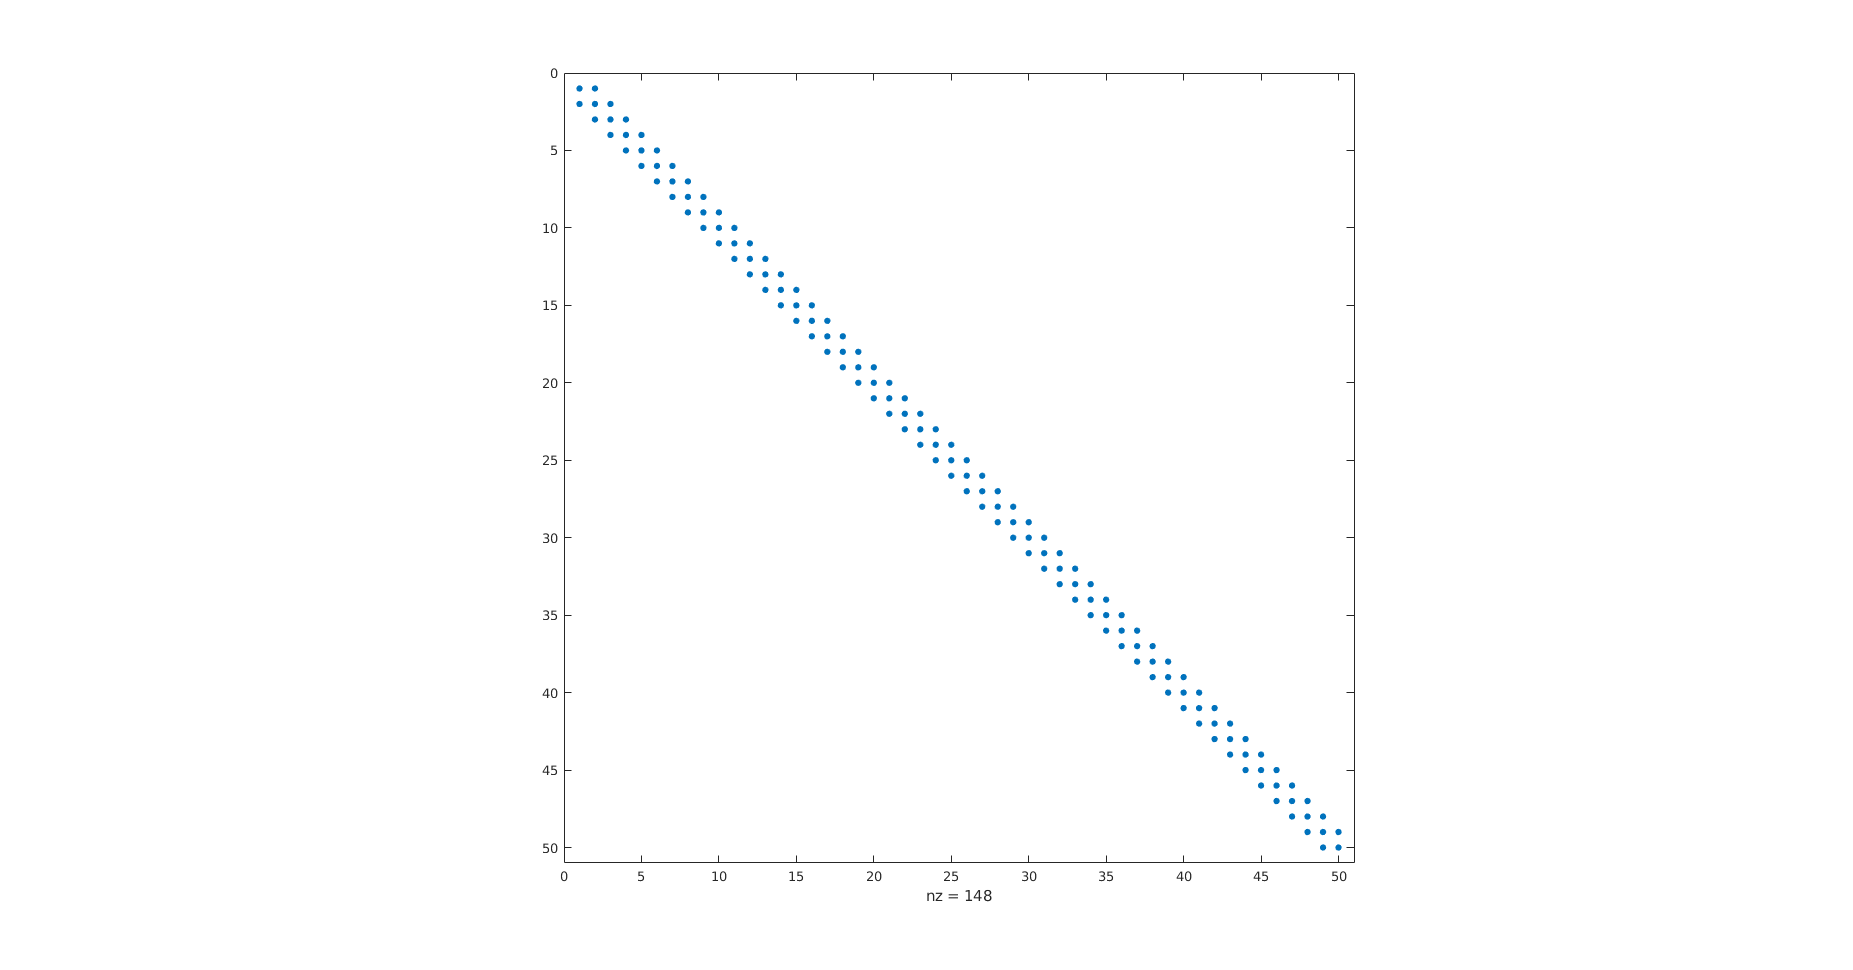
\includegraphics[scale=0.30]{1d50.png}
  \end{figure}

\item
  $d=2, k=10$. The diagonal entries are $-4$,
  and all other nonzero entries are $1$.
    \begin{figure}[H]
    \centering
    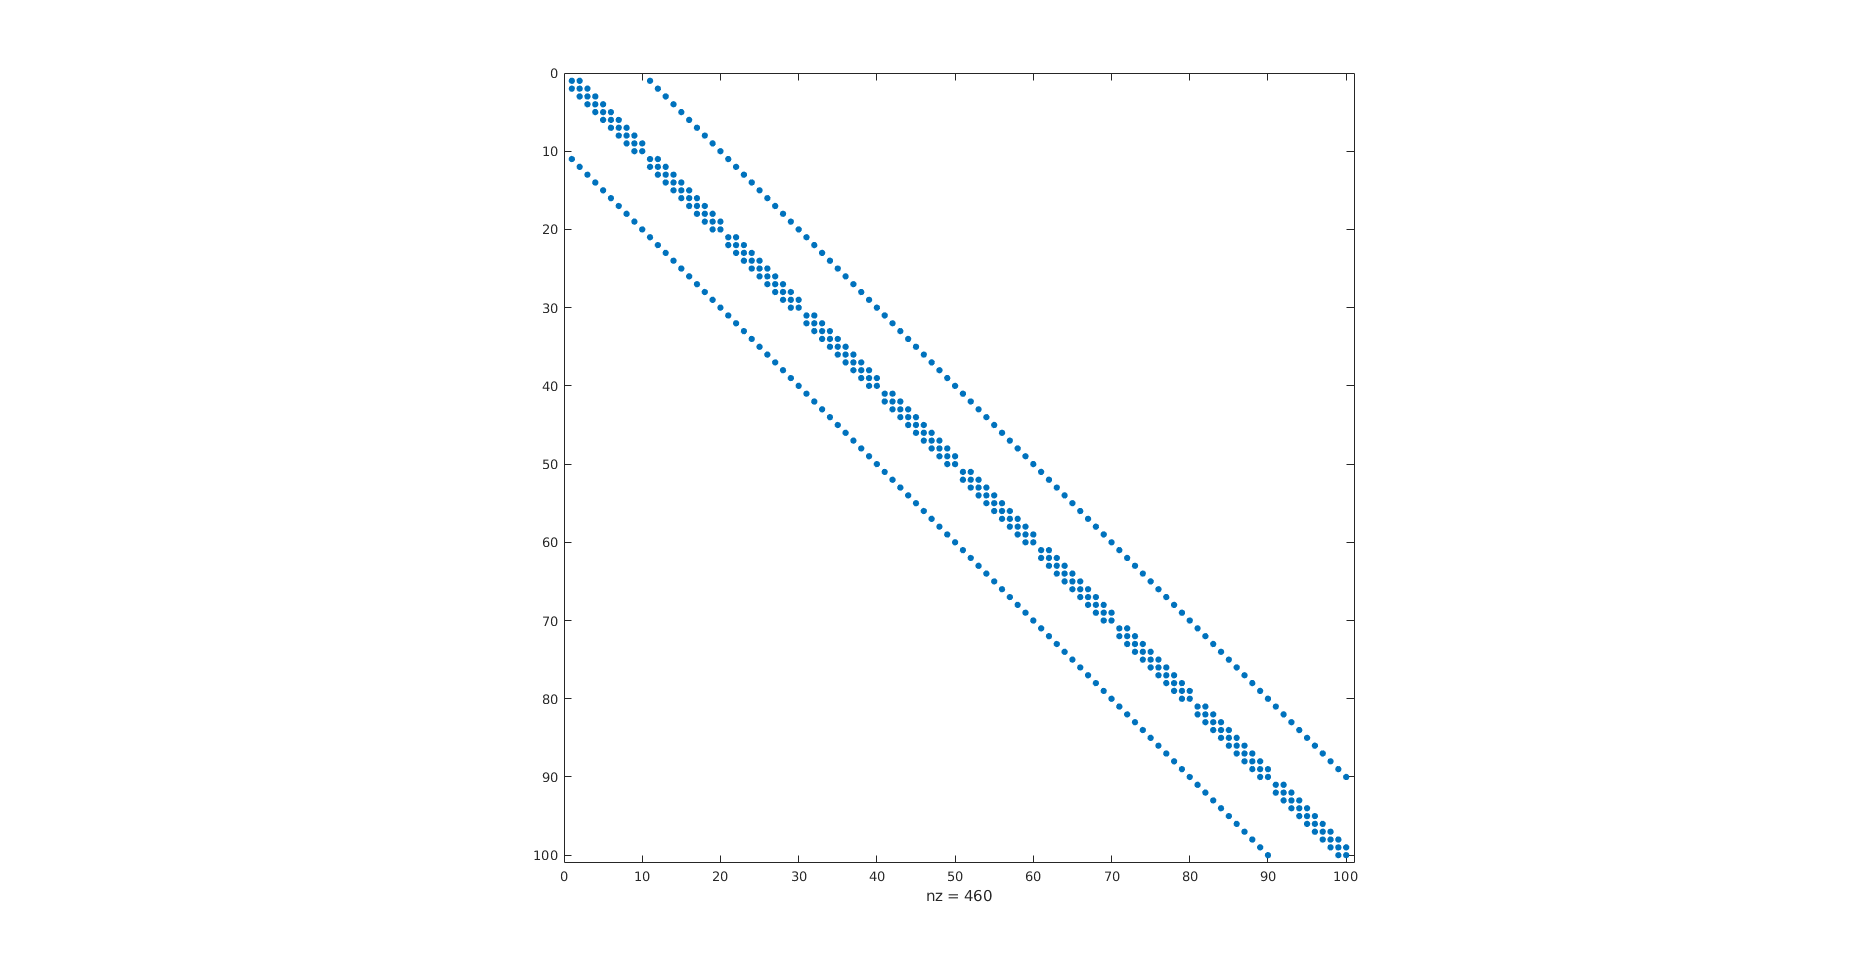
\includegraphics[scale=0.25]{2d10.png}
  \end{figure}

\item
  $d=3, k=5$. The diagonal entries are $-8$,
  and all other nonzero entries are $1$.
    \begin{figure}[H]
    \centering
    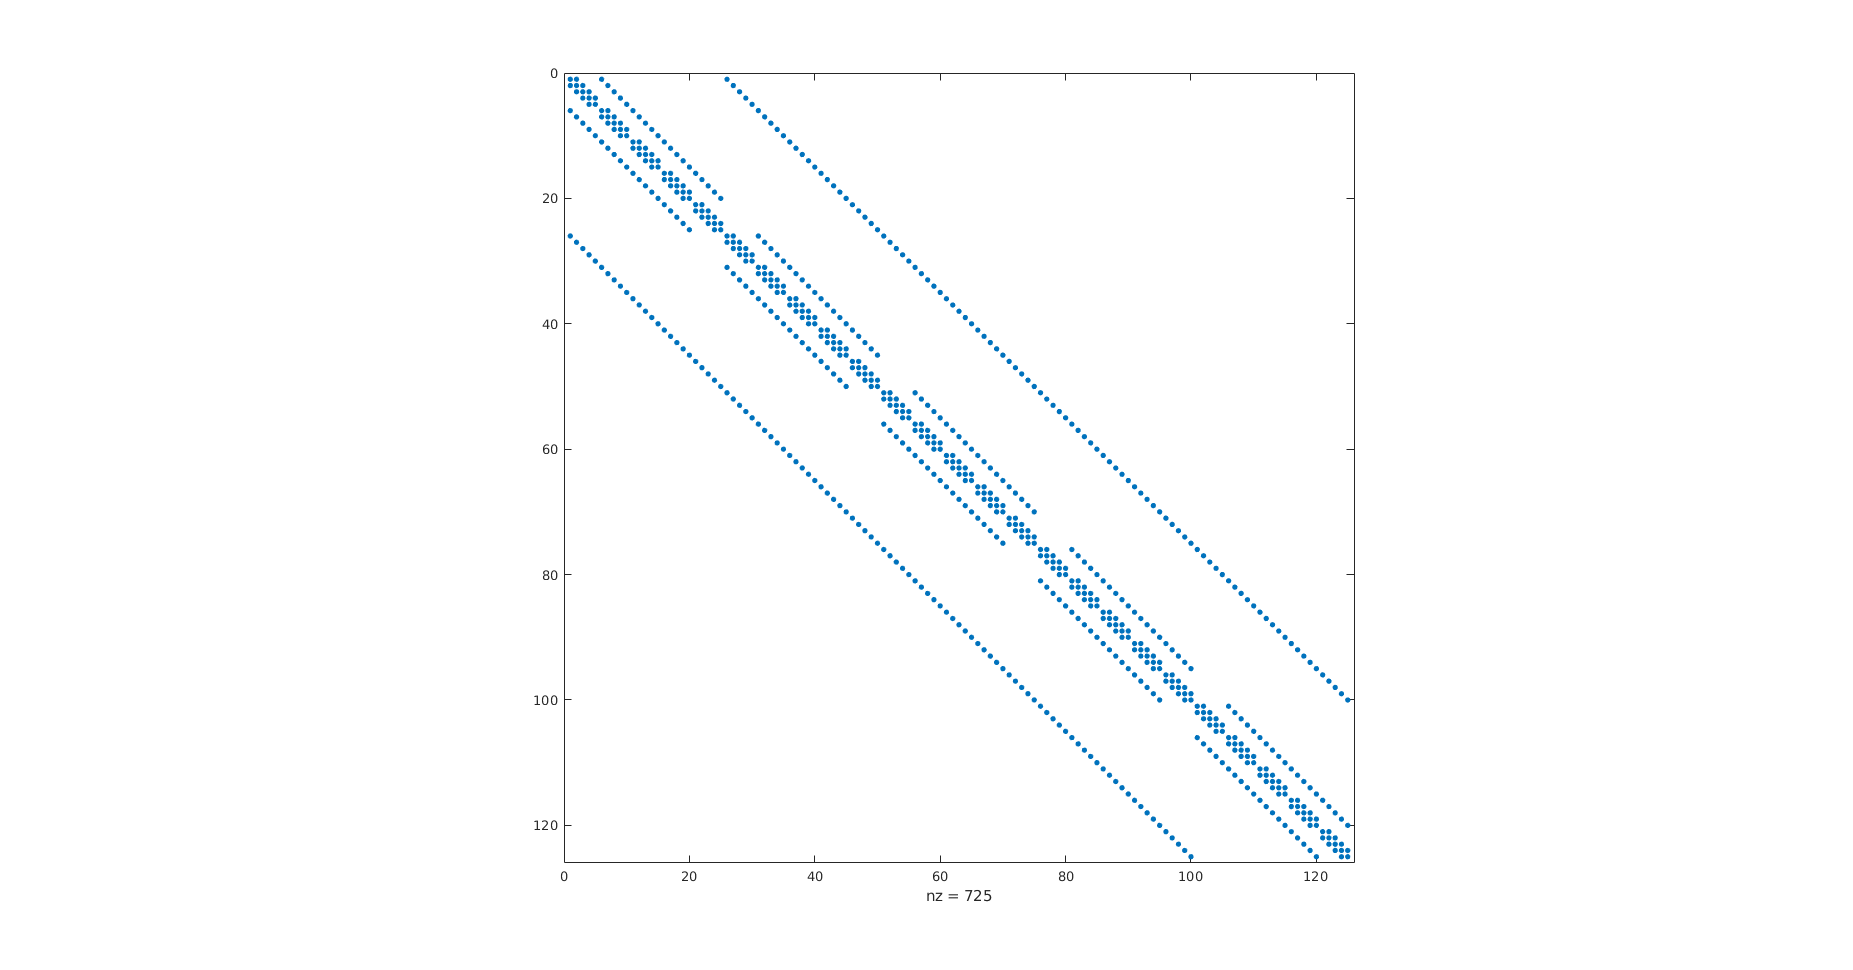
\includegraphics[scale=0.25]{3d5.png}
  \end{figure}
  \end{itemize}
\end{sol}
%%% Local Variables:
%%% mode: latex
%%% TeX-master: "../hw5"
%%% End:
